\chapter{Implementation: the SoundSuggest application}\label{chapter:implementation}

The application that was built for this thesis is called \emph{SoundSuggest}. It is a chrome extension that uses the D3 JavaScript library and the Last.fm API to inject the explanation system into the recommendations page of Last.fm\footnote{\url{http://www.last.fm/home/recs}}. In this chapter we will discuss the technologies we have used to create the application, the software design of the application and some specifics about the implementation of the application.


\section{Technologies}\label{chapter:implementation:section:technologies}

\subsection{Chrome extensions}\label{chapter:implementation:section:technologies:subsection:chrome}

Chrome Extensions are applications written in \emph{HTML}\index{HTML}, \emph{JavaScript}\index{JavaScript} and \emph{CSS}\index{CSS}\index{Cascading style sheet|see{CSS}}, that enhance to functionality of the Google Chrome web browser\cite{google:2012:extensions}.

There are different types of extensions. Browser actions are applications that can be launched regardless of the web page you are at. They appear as a button with a specified logo in the toolbar of the Chrome browser. By clicking the browser action you can specify to open up a tooltip or a popup\cite{google:2012:browseraction}. Page action extensions are meant to be shown when browsing specific web pages. They appear as an icon in the address bar. Page actions use content scripts to inject code into the web page\cite{google:2012:overview}.

The file \texttt{manifest.JSON} is one of the key areas of a chrome extension. It specifies the name and the version of your application as well as other important settings such as the type of the extension, scripts and security policies\cite{google:2012:manifest}.

Many extensions use a two-layered structure in which you have a background page and UI pages or content scripts\cite{google:2012:overview}. In the usual case the views are stateless and background pages are not. When the view needs some state, it requests the state from the background page. When the background page notices a state change, the background page tells the views to update\cite{google:2012:background}. Background pages can either be persistent or not. In the last case we are talking about so called event pages; they are opened and closed as needed\cite{google:2012:overview}.

There are various ways to use UI pages: you can open an HTML page in a popup, another tab or options page. The HTML pages inside an extension have complete access to each other's DOMs, and they can invoke functions on each other\cite{google:2012:overview}.

Content scripts are JavaScript scripts that are used to interact with a webpage opened in a browser tab. An important remark is that you should consider a content script part of the webpage it is injected into, rather than its parent extension. It can modify the DOM of the webpage but not the DOM of its background page. However it can ask its background page for data through listeners in the background page's script\cite{google:2012:overview}.



\subsection{The Last.fm API}\label{chapter:implementation:section:technologies:subsection:lastfm}

The \emph{Last.fm API}\index{Last.fm API}\index{Last.fm}\footnote{\url{http://www.last.fm/api}} offers great functionality such as the recommender system, Last.fm scrobbling and accessing and modifying your Last.fm profile information, aside from providing a large amount of data. To use the API, libraries have been developed for several technologies, such as \emph{JavaScript}\index{JavaScript}, \emph{PHP}, \emph{Python} and \emph{Actionscript} among others\cite{lastfm:2012:home}.

To build an application using the Last.fm API, you have to create an API account first at \url{http://www.last.fm/api/account/create}. Once you have been registered, you will receive an API key and an API secret.

For testing purposes it will also be handy to have a Last.fm account of your own. So if you haven't got one already sign up at their website. You might also want to one or more of their \emph{Scrobbler}\index{Scrobbler} applications. This will collect data from your music players to generate profile information that will be used to generate recommendations\cite{lastfm:2013:scrobbling}.

There are already several interesting applications that make use of the Last.fm API\index{Last.fm API}. Even more interesting perhaps is that some developers distribute free JavaScript libraries that act like a facade on the Last.fm API. The JavaScript library we will be using here, can be found on \emph{GitHub}\footnote{\url{https://github.com/fxb/javascript-last.fm-api}} and is written by \emph{Felix Bruns}.


\subsection{D3.js JavaScript Library}\label{chapter:implementation:section:technologies:subsection:d3js}

Visualizations for web applications can be built using \emph{scalable vector graphics}\index{scalable vector graphics} \emph{(SVG)\index{SVG|see{scalable vector graphics}}}. SVG is an XML-based language to describe two-dimensional graphics\cite{w3c:2011:svg}. It is supported by most of the latest versions of most popular browsers, including \emph{Chrome}, \emph{Firefox}, \emph{Internet Explorer 9}, \emph{Opera} and \emph{Safari}\cite{microsoft:2012:svg, w3c:2010:svg}.

\emph{D3.js}\index{D3.js} is a JavaScript library that uses the W3C standards \emph{HTML}, \emph{SVG} and \emph{CSS} to build data-driven documents\index{data-driven documents|see{D3.js}}\cite{bostock:2012:d3js}. There are various tutorials explaining the basics on how to use this library.

In short, to get started the library should be included in your web page. Next, using the D3 selectors, elements can be added and removed easily from the web page. The library also offers a number of built-in algorithms, as well as a series of example visualizations that can be customized as desired.


\subsection{Additional libraries}\label{chapter:implementation:section:technologies:subsection:libs}

In addition to the Last.fm API JavaScript library and D3.js, four other JavaScript libraries were used, namely:

\begin{itemize}
	\item \textbf{jQuery}\footnote{\url{http://jquery.com/}}\index{jQuery}: "jQuery is a fast, small, and feature-rich JavaScript library. It makes things like HTML document traversal and manipulation, event handling, animation, and Ajax much simpler with an easy-to-use API that works across a multitude of browsers"\cite{jquery:2013}.
	\item \textbf{jQuery UI}\footnote{\url{}}: "jQuery UI is a curated set of user interface interactions, effects, widgets, and themes built on top of the jQuery JavaScript Library"\cite{jqueryui:2013}.
	\item \textbf{Purl.js}\footnote{\url{https://github.com/allmarkedup/jQuery-URL-Parser}}: a library built on the jQuery library to retrieve GET parameters from the web page's URL.
	\item \textbf{Spinner.js}\footnote{\url{http://fgnass.github.io/spin.js/}}: a library that creates a spinner element with given parameters for customization.
\end{itemize}


\section{Software design and application architecture}\label{chapter:implementation:section:design}

The architecture of the application is shown in figure \ref{fig:architecture}. Five distict components can be identified that are of importance for the application:

\begin{itemize}
	\item \textbf{Last.fm recommendations page}: The HTML will we injected into this page. Although it is not a part of the source code, it poses certain limitations on the script. For example one should be careful not to override certain CSS definitions, and the injected code should fit into the page layout to achieve better looking results.
	\item \textbf{Content script}: The content script creates the injected HTML elements, handles user input, and delegates calls to the Last.fm API to the background script.
	\item \textbf{Background script}: the background script deals with local storage and calls to the Last.fm API.
	\item \textbf{Local storage}: The local storage of the Chrome browser can be used to store preferences.
	\item \textbf{Last.fm API}: The Last.fm API handles calls and returns the requested content.
\end{itemize}


\begin{figure}%
	\begin{center}
		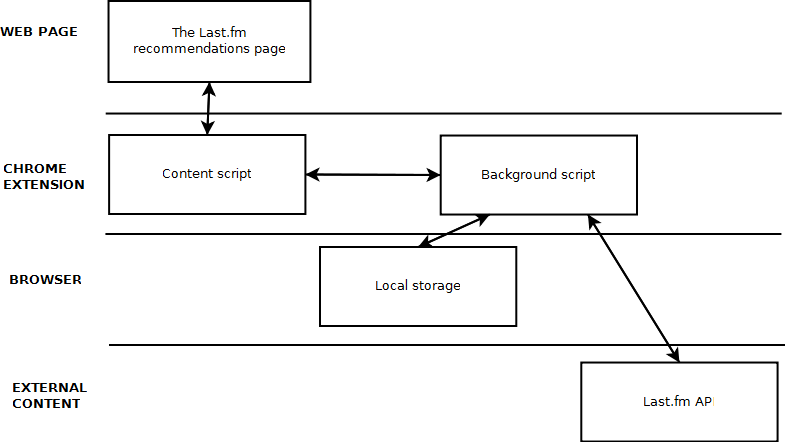
\includegraphics[width=\columnwidth]{img/architecture}%
	\end{center}
	\caption{The architecture of the application.}%
	\label{fig:architecture}%
\end{figure}

Figures \ref{fig:sequence:part1} and \ref{fig:sequence:part2} show the sequence diagrams of what happens when loading the application. The first time the application is loaded, the user will have to authenticate the application. If the user does this, the content script will retrieve the token from the callback URL, and get a session key from the Last.fm API. This session key then stored. When the application is started again, the stored key can be retrieved from the local storage. Similarly other settings are loaded from local storage. If none have been stored so far, the default settings are returned and stored.

% Life lines :
%		ACTOR
%		(UI)
%		content script
%		background script
%		Local storage
%		Last.fm API

\begin{figure}%
	\begin{center}
		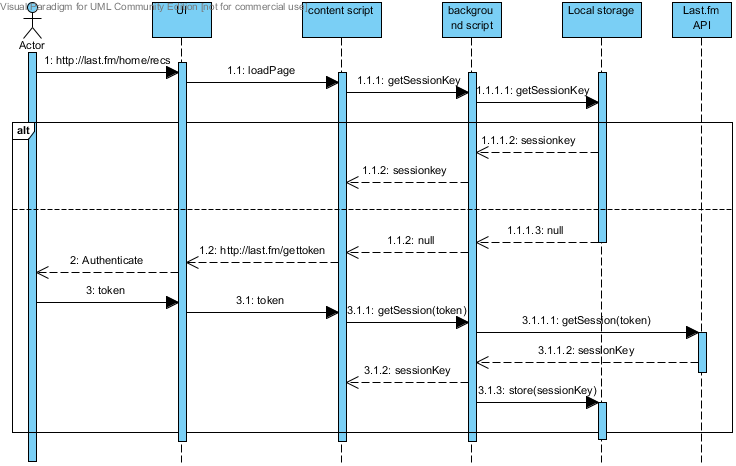
\includegraphics[width=\columnwidth]{img/seq_part1}%
	\end{center}
	\caption{Sequence diagram: opening the Last.fm recommendations page part 1: retrieving a session key.}%
	\label{fig:sequence:part1}%
\end{figure}

\begin{figure}%
	\begin{center}
		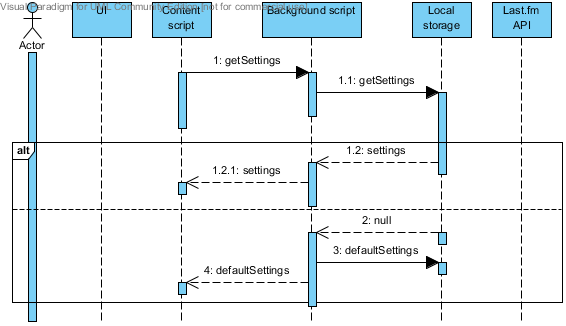
\includegraphics[width=\columnwidth]{img/seq_part2}%
	\end{center}
	\caption{Sequence diagram: opening the Last.fm recommendations page part 2: retrieving stored settings.}%
	\label{fig:sequence:part2}%
\end{figure}


Algorithm \ref{alg:loadingvis} shows how the data structure is constructed from calls to the Last.fm API\index{Last.fm API}. The resulting data structure is an approximation of the utility matrix on a local scale, i.e., the neighbourhood of the active user and the top artists of the active user. The time complexity of the algorithm depends on the number of artists, i.e., the number of recommendations added to the number of top artists, and the number of neighbours involved The resulting time complexity is then $O((R + T) * N)$.


\begin{algorithm}[H]
		\SetAlgoLined
		\KwData{Active user $user$}
		\KwResult{Datastructure $D$}
		$D$ $\leftarrow$ $\emptyset$ \;
		$N$ $\leftarrow$ getNeighbours($user$)\;
		$U$ $\leftarrow$ union($user$, $N$)\;
		$T$ $\leftarrow$ getTopartists($user$)\;
		$R$ $\leftarrow$ getRecommendations($user$)\;
		$A$ $\leftarrow$ union($T$, $R$)\;
		% FOR EACH ARTIST
		\ForEach{artist $a$ in $A$}{
			% FOR EACH USER
			\ForEach{user $u$ in $U$}{
				$Similar$ $\leftarrow$ getSimilar($a$)\;
				$Score$ $\leftarrow$ compare(union($a$, $Similar$), $u$)\;
				% IF
				\If{$Score$ $>$ $threshold$}{
					$D$.$artistMAP$[$a$] $\leftarrow$ union($D$.$artistMAP$[$a$], $u$)\;
					$D$.$userMAP$[$u$] $\leftarrow$ union($D$.$userMAP$[$u$], $a$)\;
				}
			}
		}
	\caption{Loading the data for the visualization.}
	\label{alg:loadingvis}
\end{algorithm}


The corresponding sequence diagram is shown in figure \ref{fig:sequence:loadingvis}. The two calls within the inner loop have a large impact on the performance of the algorithm. Cashing parts of the data structure is possible. However, small changes in the data may have an impact on the rest of data structure. For example if a user gets promoted to a neighbour and another gets demoted, it is impossible to know which user has to be removed from the data structure without comparing the lists of updated neighbours to the old version. Next the relevant neighbours should be removed from the data set and the new ones added. For artists that are promoted to the status of recommendation, there is a similar scenario. In this case, note that all of the users should be compared to the new items as well.


\begin{figure}%
	\begin{center}
		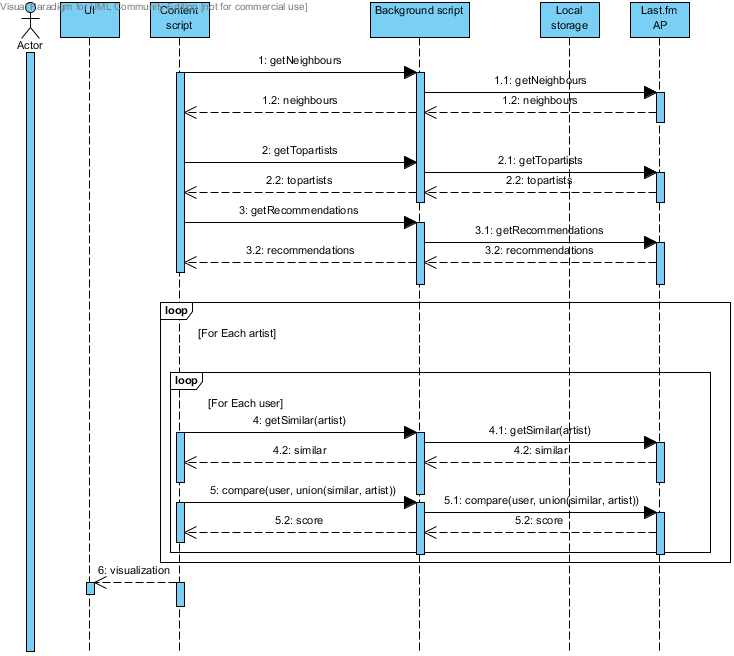
\includegraphics[width=\columnwidth]{img/seq_load_visualization}%
	\end{center}
	\caption{Sequence diagram: loading the visualization.}%
	\label{fig:sequence:loadingvis}%
\end{figure}



\section{Implementation}\label{chapter:implementation:section:implementation}

\subsection{Configuration file \texttt{manifest.JSON}}\label{chapter:implementation:section:implementation:subsection:configuration}

Aside from the basic parameters in the \texttt{manifest.JSON} file, such as \texttt{name}, \texttt{version}, \texttt{manifest\_version}, et cetera, there are several parameters that require some more attention. First of all, this extension is defined as a so-called page action. This is done by adding the page action with required attributes, namely certain icons and a default title, to the JSON file. The icon will become visible in the address bar when visiting a page defined in the \texttt{content\_scripts} parameter. In this case the script will become active when visiting the recommendations page of the \emph{Last.fm}\index{Last.fm} website. The various CSS and JavaScript used in the extension are also listed together with the content script.

As the application makes use of the storage functionality, the storage option should be added to the permissions. Since the application does calls to the Last.fm audioscrobbler, this link should be added to the permissions as well. Note that SSL is required when making external calls, otherwise the application won't even be accepted when uploading it to the chrome web store. The link should also be addded to the \texttt{content\_security\_policy} parameter of the manifest file.

To be able to access and load images, for example in the CSS definitions, it is necessary to add these to the \texttt{web\_accessible\_resources} parameter.

\subsection{The visualization \texttt{infovis}}\label{chapter:implementation:section:implementation:subsection:whitebox}

The visualization consists out of four main parts:

\begin{itemize}
	\item JSON data;
	\item JavaScript script;
	\item CSS style sheet;
	\item Custom implementation of certain methods.
\end{itemize}

\subsubsection{Data structure}

The JSON file structure is shown in listing \ref{listing:jsonfile}. It consists out of a list of artists and users that were retrieved using algorithm \ref{alg:loadingvis}. It can be generated by using the output of algorithm \ref{alg:loadingvis} as input for algorithm \ref{alg:createjson}.

\lstinputlisting[language=javascript, caption=The structure of the JSON file that is the input for the visualization script., label=listing:jsonfile]{src/datastructure.json}

%FOR EACH a IN dataArtists.keys
%	FOR EACH u IN artistData.get (a)
%		FOR d IN userData.get (u)
%			JSON.append ("edges", "item." + d.name + ".user." + u.name)
%		END-FOR
%	END-FOR
%	artist.put ("recommendation", u == active_user)
%	artist.put ("name", "item." + a.name)
%	JSON.append ("items", artist)
%END-FOR
%
%FOR EACH u IN userData.keys
%	user.put ("name", u.name)
%	user.put ("active", u == active_user)
%	FOR EACH a IN userData.get (u)
%		user.append ("owned", "item." + a.name)
%	END-FOR
%	JSON.append ("users", user)
%END-FOR

\begin{algorithm}[H]
		\SetAlgoLined
		\KwData{Data structure $D$ from algorithm \ref{alg:loadingvis}, active user $active$.}
		\KwResult{JSON file $JSON$ as in listing \ref{listing:jsonfile}.}
		$JSON$ $\leftarrow$ $\{\}$ \;
		% artistMAP = map where artists are keys, for each key there is a list of users.
		% FOR EACH ARTIST
		\ForEach{Artist $a$ in $D$.$artistMap$.$keys$}{
			$artist$ $\leftarrow$ $\{\}$ \;
			$artist$.put ("name", "item." + $a$.$name$)\;
			$isrecommendation$ $\leftarrow$ false \;
			% FOR EACH USER
			\ForEach{User $u$ in $D$.$artistMap$[$a$]}{
				% userMAP = map where users are keys, for each key there is a list of artists.
				\If{$u$.equals ($active$)}{
					$isrecommendation$ $=$ true\;
				}
				\ForEach{Artist $d$ in $D$.$userMap$[$u$]}{
					$artist$.append ("edges", "item." + $d$.$name$ + ".user." + $u$.$name$)\;
				}
			}
			$artist$.put ("recommendation", $isrecommendation$)\;
			$JSON$.append ($artist$)\;
		}
		\ForEach{User $u$ in $D$.$userMap$.$keys$}{
				% FOR EACH USER
				$user$ $\leftarrow$ $\{\}$ \;
				$user$.put ("name", $u$.$name$)\;
				$user$.put ("active", $u$.equals ($active$))\;
				% userMAP = map where users are keys, for each key there is a list of artists.
				\ForEach{Artist $d$ in $D$.$userMap$[$u$]}{
					$user$.append ("owned", "item." + $d$.$name$)
				}
				$JSON$.append ($user$)\;
			}
		}
	\caption{Loading the data for the visualization.}
	\label{alg:createjson}
\end{algorithm}


\subsubsection{The visualization script}

Once the data structure has been constructed, it is plugged into the script. Listing \ref{listing:createwhitebox} shows how this is done in JavaScript, assuming that the variables $LAYOUT$ and $DATA$ are known. The script uses the data to generate nodes, edges in an \texttt{SVG} element, and a list of users as \texttt{LI} elements in an \texttt{UL} element next to the visualization.

For this visualization, a D3.js hierarchical edge-bundling example by Michael Bostock was adapted. The major changes to the original code are the extension of the original data structure as explained in the previous section, and the addition of extra CSS classes to support interactions with the user list, which are discussed in the next section. In conclusion, for a detailed description of the visualization code, we refer to the D3.js website\footnote{The original code of the hierarchical edge-bundling example can be found at \url{http://bl.ocks.org/mbostock/1044242}.}.


\lstinputlisting[language=javascript, caption=Create a new Whitebox object for given settings and data., label=listing:createwhitebox]{src/create_whitebox.js}

\subsubsection{Style sheet}

To support hover and click interactions, each node and each user \texttt{LI} element has an \emph{onmouseover}, \emph{onmouseout}, and \emph{click} event listener attached to it. When one of these events is triggered, the appropriate classes are added or removed from these elements. Table \ref{table:interactions} shows which classes are activated for which interaction. Each of these classes in also combined with another set of classes as listed in table \ref{table:colours}. By changing the colour classes for nodes, edges and \texttt{LI}'s, colour patterns chosen by the end user are applied on the fly.


\begin{table}%
	\begin{center}
		\begin{tabular}{l | l l}
			\hline
			\textbf{Interaction}		& SVG Node in \textbf{\#chart svg} & User LI in \textbf{ul\#users }
			\\
			\hline
			Click node		& \textit{.link-item-clicked} & \textit{.user-item-clicked} \\
										& \textit{.node-item-clicked} & \\
			Click user		& \textit{.user-clicked} 			& \textit{.user-clicked} \\
										& \textit{.link-user-clicked} & \\
										& \textit{.node-user-clicked} & \\
			Hover node		& \textit{.node-item-mouseover} 	& \textit{.user-item-mouseover} \\
										& \textit{.user-item-mouseover}		& \\
			Hover user		& \textit{.node-user-mouseover} 	& \textit{.user.user-mouseover} \\
										& \textit{.link-user-mouseover}		& \\
			\hline
		\end{tabular}
	\end{center}
	\caption{Overview of the classes that added for each supported interaction for each interaction target.}
	\label{table:interactions}
\end{table}


\begin{table}%
	\begin{center}
		\begin{tabular}{l | l l l}
			\hline
			& \textbf{Blue}		& \textbf{Green} & \textbf{Red}
			\\
			\hline
			Active user &	\textit{.blue-active}	& \textit{.green-active} & \textit{.red-active} \\
			Mouseover 	&	\textit{.blue-mouseover}	& \textit{.green-mouseover} & \textit{.red-mouseover} \\
			Click				&	\textit{.blue-clicked}	& \textit{.green-clicked} & \textit{.red-clicked} \\
			\hline
		\end{tabular}
	\end{center}
	\caption{Overview of the classes that added for each supported colour.}
	\label{table:colours}
\end{table}




